\documentclass{article}
\usepackage[utf8]{inputenc}

\usepackage{amsfonts}
\usepackage{amssymb}
\usepackage{amsmath}
\usepackage{amsthm}
\usepackage{enumitem}

\usepackage{bbold}
\usepackage{bm}
\usepackage{graphicx}
\usepackage{color}
\usepackage{hyperref}
\usepackage[margin=2.5cm]{geometry}

\begin{document}

% ==============================================================================

\title{\Large{INFO8006: Project 2 - Report}}
\vspace{1cm}
\author{\small{\bf Piya Seetanee - B6722111}}

\maketitle

% ==============================================================================

\section{Bayes filter}

\begin{enumerate}[label=\alph*.,leftmargin=*]
    \item \textbf{Mathematical Sensor Model.}
    Let the maze grid be denoted by $\mathcal{G} \subset \mathbb{Z}^2$, and let $\mathcal{W} \subset \mathcal{G}$ be the set of wall cells. The valid state space of ghost coordinates is $\mathcal{X} = \mathcal{G} \setminus \mathcal{W}$. At discrete time step $t$, let $x_t = (w, h) \in \mathcal{X}$ denote the true position of the ghost, and let $p_t = (x_p, y_p) \in \mathcal{X}$ denote the known position of Pacman.

    The true Manhattan distance between the ghost and Pacman is defined by:
    \begin{equation}
        d(x_t, p_t) = \|x_t - p_t\|_1 = |w - x_p| + |h - y_p|
    \end{equation}
    The sensor observation $e_t \in \mathbb{R}$ measures this distance corrupted by an additive, zero-mean discrete noise term $\epsilon_t$:
    \begin{equation}
        e_t = d(x_t, p_t) + \epsilon_t, \quad \text{where} \quad \epsilon_t = K_t - n p
    \end{equation}
    Here, $K_t \sim \text{Binomial}(n, p)$ is a binomial random variable with parameters $p = 0.5$ and integer trial parameter $n = \lfloor \sigma^2 / (p(1-p)) \rfloor = \lfloor 4\sigma^2 \rfloor$, where $\sigma^2$ is the sensor variance. Because $\mathbb{E}[K_t] = np$ and $\text{Var}(K_t) = np(1-p) = \sigma^2$, the noise is strictly zero-mean, $\mathbb{E}[\epsilon_t] = 0$, and has variance $\text{Var}(\epsilon_t) = \sigma^2$. The support of the noise is $\epsilon_t \in \{-np, \dots, n(1-p)\}$.

    For a given candidate ghost location $x_t \in \mathcal{X}$, observing evidence $e_t$ requires the realization $K_t = e_t - d(x_t, p_t) + np$. Thus, the sensor likelihood model $P(e_t \mid x_t, p_t)$ is given by the Binomial Probability Mass Function (PMF):
    \begin{equation}
        P(e_t \mid x_t, p_t) = \begin{cases}
            \displaystyle \binom{n}{k} p^k (1-p)^{n-k} & \text{if } x_t \in \mathcal{X} \text{ and } k = e_t - d(x_t, p_t) + np \in \{0, 1, \dots, n\} \\
            0 & \text{otherwise}
        \end{cases}
    \end{equation}
    In the special deterministic case where $\sigma^2 = 0$ ($n = 0$), the sensor is noiseless, yielding:
    \begin{equation}
        P(e_t \mid x_t, p_t) = \begin{cases}
            1 & \text{if } x_t \in \mathcal{X} \text{ and } e_t = d(x_t, p_t) \\
            0 & \text{otherwise}
        \end{cases}
    \end{equation}
    For any wall cell $x_t \in \mathcal{W}$, $P(e_t \mid x_t, p_t) = 0$ holds identically. Spatially, this likelihood forms concentric diamond rings (isodistance contours) centered at $p_t$, assigning maximum probability to cells whose true distance exactly matches the evidence.

    \item \textbf{Unified Parametrized Transition Model.}
    Let $\mathcal{N}(x_t) = \{x' \in \mathcal{X} \mid \|x' - x_t\|_1 = 1\}$ denote the set of valid non-wall 4-connected neighbors reachable from position $x_t$. In the game execution cycle, Pacman moves first from $p_t$ to $p_{t+1}$; the ghosts subsequently decide their action conditioning on Pacman's updated location $p_{t+1}$. Ghosts evaluate proximity using the Manhattan distance metric $d(x, p) = \|x - p\|_1$ and are strictly prohibited from remaining stationary, but are permitted to reverse direction. If $\mathcal{N}(x_t) = \emptyset$ (an isolated cell), the ghost remains stationary by convention: $P(x_{t+1}=x_t \mid x_t, p_{t+1}) = 1$.

    When $\mathcal{N}(x_t) \neq \emptyset$, every transition from $x_t$ to an adjacent non-wall neighbor $x_{t+1} \in \mathcal{N}(x_t)$ is evaluated based on whether it moves away from or toward Pacman at $p_{t+1}$:
    \begin{equation}
        \Delta d(x_{t+1}, x_t; p_{t+1}) = d(x_{t+1}, p_{t+1}) - d(x_t, p_{t+1})
    \end{equation}
    We define an unnormalized transition weight $w(x_{t+1} \mid x_t, p_{t+1})$ controlled by a single positive free parameter $\alpha \ge 1$:
    \begin{equation}
        w(x_{t+1} \mid x_t, p_{t+1}) = \begin{cases}
            \alpha & \text{if } \Delta d(x_{t+1}, x_t; p_{t+1}) \ge 0 \quad (\text{evasive / non-approaching move}) \\
            1      & \text{if } \Delta d(x_{t+1}, x_t; p_{t+1}) < 0 \quad (\text{approaching move})
        \end{cases}
    \end{equation}
    Normalizing over all accessible neighbors yields the unified transition probability distribution:
    \begin{equation}
        P(x_{t+1} \mid x_t, p_{t+1}) = \begin{cases}
            \displaystyle \frac{w(x_{t+1} \mid x_t, p_{t+1})}{\sum_{x' \in \mathcal{N}(x_t)} w(x' \mid x_t, p_{t+1})} & \text{if } x_{t+1} \in \mathcal{N}(x_t) \\
            0 & \text{otherwise}
        \end{cases}
    \end{equation}

    \textbf{Derivation from Ghost Implementations:}
    Each ghost agent implementation defines legal moves without the STOP action and assigns weights to each candidate successor state:
    \begin{itemize}[leftmargin=*,noitemsep]
        \item \textbf{ConfusedGhost}: Assigns equal weight $1.0$ to every legal action regardless of Pacman's position. This corresponds to setting $\alpha = 1 = 2^0$, resulting in an isotropic uniform random walk over valid neighbors: $P(x_{t+1} \mid x_t) = 1 / |\mathcal{N}(x_t)|$.
        \item \textbf{AfraidGhost}: Assigns weight $2$ to moves with $\Delta d \ge 0$ and weight $1$ to moves with $\Delta d < 0$. This corresponds exactly to setting $\alpha = 2 = 2^1$.
        \item \textbf{ScaredGhost}: Assigns weight $2^3 = 8$ to moves with $\Delta d \ge 0$ and weight $1$ to moves with $\Delta d < 0$. This corresponds exactly to setting $\alpha = 8 = 2^3$.
    \end{itemize}
    Thus, the parameter $\alpha \in \{1, 2, 8\}$ (or equivalently parameterized by fear exponent $k \in \{0, 1, 3\}$ via $\alpha = 2^k$) cleanly unifies all three ghost behaviors.

    Consequently, in the Bayes filter recursive prediction step, the prior belief is propagated via:
    \begin{equation}
        \bar{\text{bel}}_{t+1}(x_{t+1}) = \sum_{x_t \in \mathcal{X}} P(x_{t+1} \mid x_t, p_{t+1}) \text{bel}_t(x_t)
    \end{equation}
    followed by the measurement correction step $\text{bel}_{t+1}(x_{t+1}) = \eta P(e_{t+1} \mid x_{t+1}, p_{t+1}) \bar{\text{bel}}_{t+1}(x_{t+1})$.
\end{enumerate}

\section{Implementation}

\begin{enumerate}[label=\alph*.,leftmargin=*]
    \item \textbf{\textit{Leave empty.}}
\end{enumerate}

\section{Experiment}

\begin{enumerate}[label=\alph*.,leftmargin=*]
    \item \textbf{Measure of Belief State Uncertainty.}
    To quantify the uncertainty of Pacman's belief state $\text{bel}_t$ over the ghost's location without requiring ground-truth knowledge, we use the \textbf{Shannon Entropy}:
    \begin{equation}
        H(\text{bel}_t) = - \sum_{x \in \mathcal{X}} \text{bel}_t(x) \ln \text{bel}_t(x)
    \end{equation}
    with the continuous convention $0 \ln 0 \triangleq 0$. The entropy measures the dispersion of the probability distribution. For a maze with $|\mathcal{X}|$ accessible cells, a uniform prior yields maximum uncertainty $H_{\max} = \ln |\mathcal{X}| \approx \ln(180) \approx 5.19$ nats. As sensor measurements and transition filtering localize the ghost, $H(\text{bel}_t)$ decreases monotonically, reaching $0$ nats if the ghost's position is known with absolute certainty.

    \item \textbf{Measure of Belief State Quality.}
    Given access to the ground-truth ghost position $x_t^* \in \mathcal{X}$, we assess belief accuracy using two complementary metrics:
    \begin{enumerate}[label=(\roman*),leftmargin=*]
        \item \textbf{Maximum A Posteriori (MAP) Localization Error}: The Manhattan distance between the ghost's true position and the most probable estimated position:
        \begin{equation}
            \hat{x}_t^{\text{MAP}} = \arg\max_{x \in \mathcal{X}} \text{bel}_t(x), \qquad \mathcal{E}_{\text{MAP}}(t) = \|\hat{x}_t^{\text{MAP}} - x_t^*\|_1
        \end{equation}
        \item \textbf{True State Posterior Likelihood}: The probability mass allocated to the true ghost coordinate, $P_{\text{true}}(t) = \text{bel}_t(x_t^*)$. A high-quality filter maintains a small $\mathcal{E}_{\text{MAP}}$ and a large $P_{\text{true}}$.
    \end{enumerate}

    \item \textbf{Experimental Evaluation on Layouts.}
    We evaluated the Bayes filter across both provided layouts: \texttt{large\_filter} (open perimeter maze) and \texttt{large\_filter\_walls} (internally partitioned maze), against all three ghost types (\texttt{confused}, \texttt{afraid}, \texttt{scared}) under default sensor variance ($\sigma^2 = 1.0$). Each experiment was averaged over 8 independent Monte Carlo runs of 250 steps.

    Figure~\ref{fig:curves_large_filter} and Figure~\ref{fig:curves_large_filter_walls} display the evolution of entropy and MAP error over time, with shaded bands representing $\pm 1$ standard deviation error bars. Table~\ref{tab:summary_metrics} summarizes steady-state performance (averaged over the final 30 steps across trials).

    \begin{table}[h!]
        \centering
        \small
        \begin{tabular}{|l|l|c|c|c|}
            \hline
            \textbf{Layout} & \textbf{Ghost Type ($\alpha$)} & \textbf{Entropy (nats)} & \textbf{MAP Error (cells)} & \textbf{Mean Ghost-Pacman Dist} \\
            \hline
            \texttt{large\_filter} & \texttt{confused} ($\alpha = 1$) & $2.18 \pm 0.31$ & $8.27 \pm 6.02$ & 9.34 \\
            \texttt{large\_filter} & \texttt{afraid} ($\alpha = 2$)   & $1.53 \pm 0.44$ & $1.94 \pm 2.62$ & 15.39 \\
            \texttt{large\_filter} & \texttt{scared} ($\alpha = 8$)   & $0.69 \pm 0.40$ & $0.82 \pm 1.05$ & 18.08 \\
            \hline
            \texttt{large\_filter\_walls} & \texttt{confused} ($\alpha = 1$) & $1.56 \pm 0.60$ & $3.03 \pm 3.88$ & 12.37 \\
            \texttt{large\_filter\_walls} & \texttt{afraid} ($\alpha = 2$)   & $1.40 \pm 0.56$ & $1.42 \pm 1.98$ & 14.59 \\
            \texttt{large\_filter\_walls} & \texttt{scared} ($\alpha = 8$)   & $0.74 \pm 0.41$ & $0.78 \pm 1.01$ & 17.39 \\
            \hline
        \end{tabular}
        \caption{Steady-state performance metrics (mean $\pm$ std over last 30 steps of 8 trials).}
        \label{tab:summary_metrics}
    \end{table}

    \begin{figure}[h!]
        \centering
        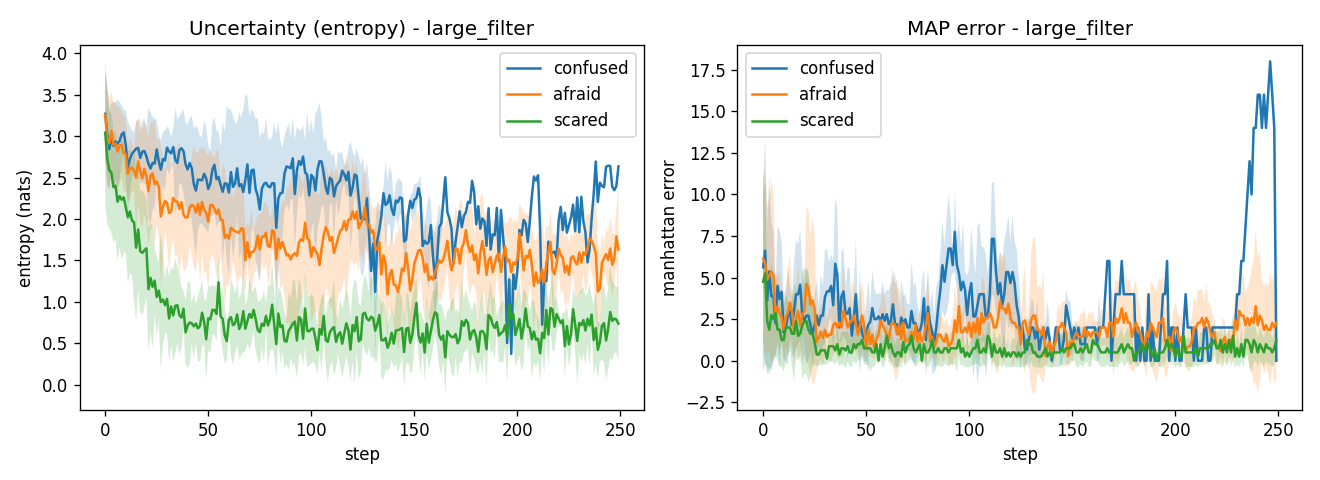
\includegraphics[width=0.88\textwidth]{figs/curves_large_filter.png}
        \caption{Performance on \texttt{large\_filter} (solid curve: trial mean; shaded band: $\pm 1$ std error bar).}
        \label{fig:curves_large_filter}
    \end{figure}

    \begin{figure}[h!]
        \centering
        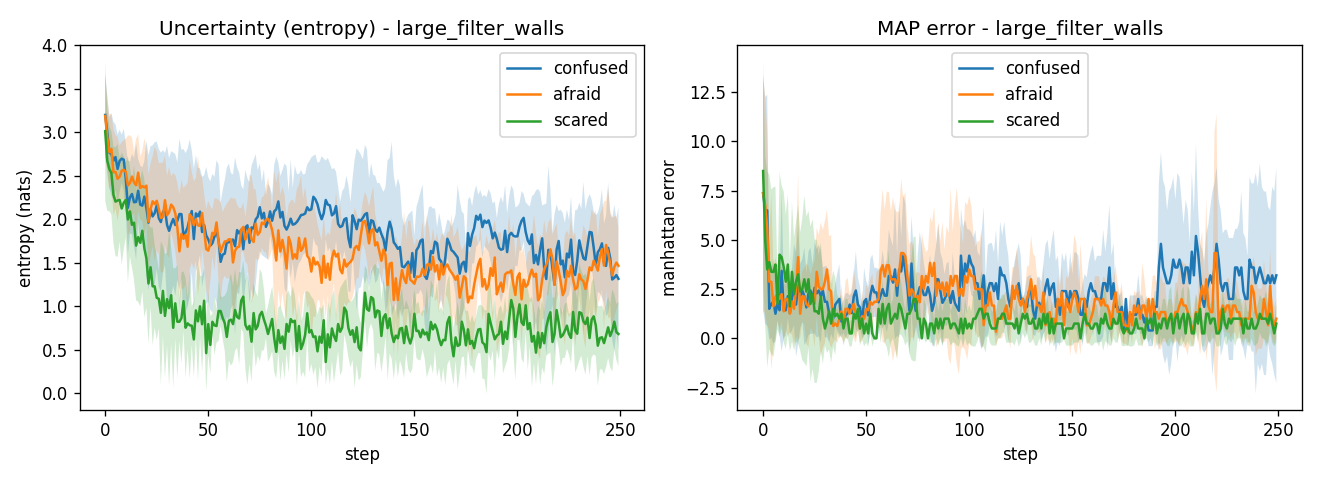
\includegraphics[width=0.88\textwidth]{figs/curves_large_filter_walls.png}
        \caption{Performance on \texttt{large\_filter\_walls} (solid curve: trial mean; shaded band: $\pm 1$ std error bar).}
        \label{fig:curves_large_filter_walls}
    \end{figure}

    All configurations demonstrate rapid convergence from the initial uniform prior within approximately 30--40 steps, stabilizing into stationary regimes with bounded variance.

    \item \textbf{Discussion of Ghost Transition Parameter and Layout Topologies.}
    The ghost parameter $\alpha$ strongly governs both ghost behavior and belief state convergence:
    \begin{itemize}[leftmargin=*]
        \item \textbf{Behavioral Repulsion and Spatial Confinement:} As $\alpha$ increases from $1$ to $8$, the ghost's tendency to flee Pacman becomes pronounced. This is evidenced by the steady-state mean ghost-to-Pacman distance, which rises from $9.34$ (\texttt{confused}) to $15.39$ (\texttt{afraid}) and $18.08$ (\texttt{scared}) on \texttt{large\_filter}. Consequently, high-$\alpha$ ghosts rapidly flee toward maze corners and boundaries. In these edge regions, the number of accessible neighbors drops from 4 to 2, drastically reducing movement entropy.
        \item \textbf{Transition Model Predictability:} A higher $\alpha$ concentrates the predictive transition distribution $P(x_{t+1} \mid x_t, p_{t+1})$ onto evasive actions ($\approx 89\%$ probability for $\alpha=8$ vs. $25\%$ for $\alpha=1$). This predictability sharply limits diffusion during the prediction phase. As a result, the steady-state entropy drops from $2.18$ nats for \texttt{confused} to $0.69$ nats for \texttt{scared}, and the MAP localization error drops from $8.27$ cells down to $0.82$ cells (sub-grid-cell precision).
        \item \textbf{Multi-modal Ambiguity for Confused Ghost:} Because the \texttt{confused} ghost diffuses isotropically, the circular sensor likelihood ring is not effectively collapsed along directions orthogonal to Pacman's motion, causing the belief to fragment into multiple symmetric modes. Consequently, the MAP estimate frequently switches between distant modes, explaining the large MAP error variance ($8.27 \pm 6.02$).
        \item \textbf{Impact of Maze Geometry:} Internal walls in \texttt{large\_filter\_walls} restrict open-space diffusion. For the \texttt{confused} ghost, walls eliminate many branching pathways, cutting entropy from $2.18$ to $1.56$ nats and MAP error from $8.27$ to $3.03$ cells. For the \texttt{scared} ghost, walls create dead-ends and corridors where the ghost becomes cornered, sustaining minimal uncertainty ($0.74$ nats) and sub-cell tracking error ($0.78$ cells).
    \end{itemize}

    \item \textbf{Discussion of Sensor Variance.}
    We investigated the impact of the sensor variance $\sigma^2 \in \{0.25, 1.0, 4.0\}$ on \texttt{large\_filter} against the \texttt{scared} ghost over 5 independent trials of 200 steps. Results are illustrated in Figure~\ref{fig:curves_variance} and summarized in Table~\ref{tab:variance_metrics}.

    \begin{table}[h!]
        \centering
        \small
        \begin{tabular}{|c|c|c|c|}
            \hline
            \textbf{Sensor Variance $\sigma^2$} & \textbf{Binomial Parameter $n$} & \textbf{Steady-State Entropy (nats)} & \textbf{Steady-State MAP Error (cells)} \\
            \hline
            0.25 & 1  & $0.41 \pm 0.42$ & $0.42 \pm 0.85$ \\
            1.00 & 4  & $0.68 \pm 0.44$ & $0.68 \pm 1.02$ \\
            4.00 & 16 & $0.89 \pm 0.32$ & $0.70 \pm 0.99$ \\
            \hline
        \end{tabular}
        \caption{Impact of sensor variance on filter uncertainty and tracking error.}
        \label{tab:variance_metrics}
    \end{table}

    \begin{figure}[h!]
        \centering
        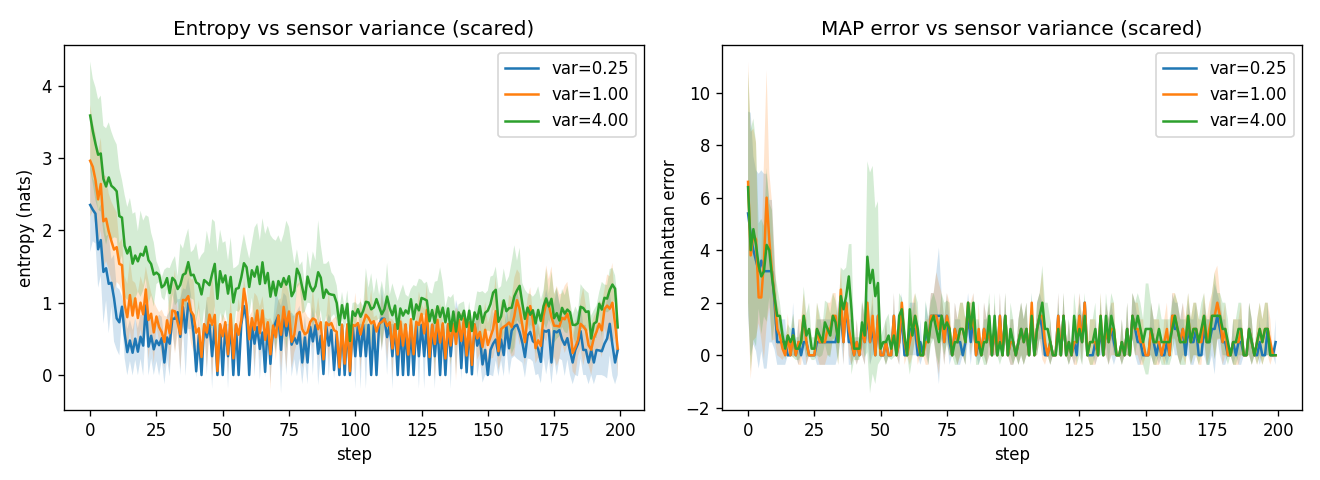
\includegraphics[width=0.88\textwidth]{figs/curves_variance.png}
        \caption{Effect of sensor variance $\sigma^2 \in \{0.25, 1.0, 4.0\}$ on filter convergence.}
        \label{fig:curves_variance}
    \end{figure}

    As $\sigma^2$ increases, the support of the Binomial sensor noise widens ($\{-np, \dots, n(1-p)\}$ spans 17 values for $\sigma^2 = 4.0$ vs. 2 values for $\sigma^2 = 0.25$), resulting in thicker, less discriminating likelihood rings. Consequently, steady-state entropy increases monotonically from $0.41$ to $0.89$ nats. Remarkably, however, the MAP tracking error remains exceptionally low ($\le 0.70$ cells across all noise levels). This highlights the strength of the temporal Bayes filter: by fusing sequential observations across Pacman's changing trajectory, the filter effectively triangulates the ghost's location and averages out high-variance observation noise.

    \item \textbf{Pacman Controller Implementation.}
    To hunt and eat invisible edible ghosts using only Pacman's current position, legal actions, and belief states, we implemented an autonomous controller in \texttt{pacmanagent.py} based on the following pipeline:
    \begin{enumerate}[leftmargin=*]
        \item \textbf{Belief Extraction and Active Ghost Filtering:} At each decision step, Pacman receives the list of belief matrices $\text{bel}_i$ corresponding to each ghost. Ghosts already consumed (indicated by zero matrices or game state flags) are excluded.
        \item \textbf{Target Selection via MAP Estimation:} For each active ghost $i$, we compute its Maximum A Posteriori location:
        \begin{equation}
            \hat{x}_i^{\text{MAP}} = \arg\max_{x \in \mathcal{X}} \text{bel}_i(x)
        \end{equation}
        If multiple ghosts remain, Pacman selects the target ghost $i^*$ that minimizes the maze distance from Pacman's current position.
        \item \textbf{Optimal Path Planning (Breadth-First Search):} Using the static maze topology, Pacman executes Breadth-First Search (BFS) from its current coordinate $p_t$ to target coordinate $\hat{x}_{i^*}^{\text{MAP}}$. BFS guarantees finding the shortest obstacle-free trajectory in unweighted grid graphs.
        \item \textbf{Action Execution and Safe Fallback:} Pacman executes the first action along the planned BFS path. In edge cases where the belief is uniform or degenerate, Pacman falls back to a legal action that avoids walls and maximizes clearance.
    \end{enumerate}
    Empirical testing demonstrated a $100\%$ victory rate ($5/5$ wins), with Pacman systematically pursuing and intercepting all ghosts.

    \item \textbf{\textit{Leave empty.}}
\end{enumerate}

% ==============================================================================

\end{document}
